\chapter{Research methods}
\chlab{methods}

The main question that this research project will try to answer is the following:
\begin{quote}
How can chemists best interact with a tool for fragment-based molecule parameterisation, such that this yields results of comparable quality to conventional methods, while being done faster?
\end{quote}
In order to answer this question, such tool will be designed and a prototype of it will be implemented. User studies will be conducted to evaluate the tool's design and results. In those studies, the results obtained by using the tool will be compared to those obtained using conventional methods, i.e. complex quantum mechanical calculations~(see~\chref{problems}).


\section{The tool}
\seclab{tool}

% TODO: why web?!
The requirements of the molecule parameterisation tool have been specified in \chref{problems}. It has been decided to implement the tool in \verb|HTML5| and \verb|JavaScript|, which allows for great portability and availability across different operating systems and platforms. It also makes the tool future-proof, by following the current trend of bringing everything to the web.

Not surprisingly, there are no existing tools for fragment-based molecule parameterisation, as this is a new concept. Furthermore, no tools exist for comparing molecules - or fragments of them - either. What does exist is a wide range of tools and programs for showing and editing molecules. This includes stand-alone molecule drawing software such as \verb|Accelerys Draw|~\cite{accelrys2012accelrys} and \verb|Avogadro|~\cite{hanwell2012avogadro}, two-dimensional web-based molecule editors like \verb|ChemDoodle 2D Sketcher|~\cite{ichemlabs2013chemdoodle}, \verb|Molsoft HTML5 Molecule Editor|~\cite{molsoft2012molsoft} and \verb|Marvin for JavaScript|~\cite{chemxon2013marvin}, and online three-dimensional visualisation tools \verb|JSMol|~\cite{hanson2013jsmol} and \verb|CanvasMol|~\cite{altered2013canvasmol}.

These existing tools will serve as an initial guideline for the tool to be developed, and parts of their implementations may be reused. The rest of the tool, however, will need to be designed and developed from scratch. The design will follow the basic interaction design principles as posed by Norman and others~(see \secref{id_principles}), the knowledge about learing~(see \secref{id_learning}), and keep in mind the insights gained by the developers of other molecule software~(see \secref{software}).

As there is no existing software for fragment-based molecule parameterisation, there is also no baseline to which the developed tool can be compared. In order to still be able to say something about the quality of the tool, two different implementations of it will be made. There are a few axles along which this difference can be made. It could, for instance, be possible to compare the results obtained by two implementations that have a different way of visualising molecules. Visualising molecules, however, is a well-exhausted field of research, leaving very little room for new ideas.

\begin{figure}[h!]
\begin{center}
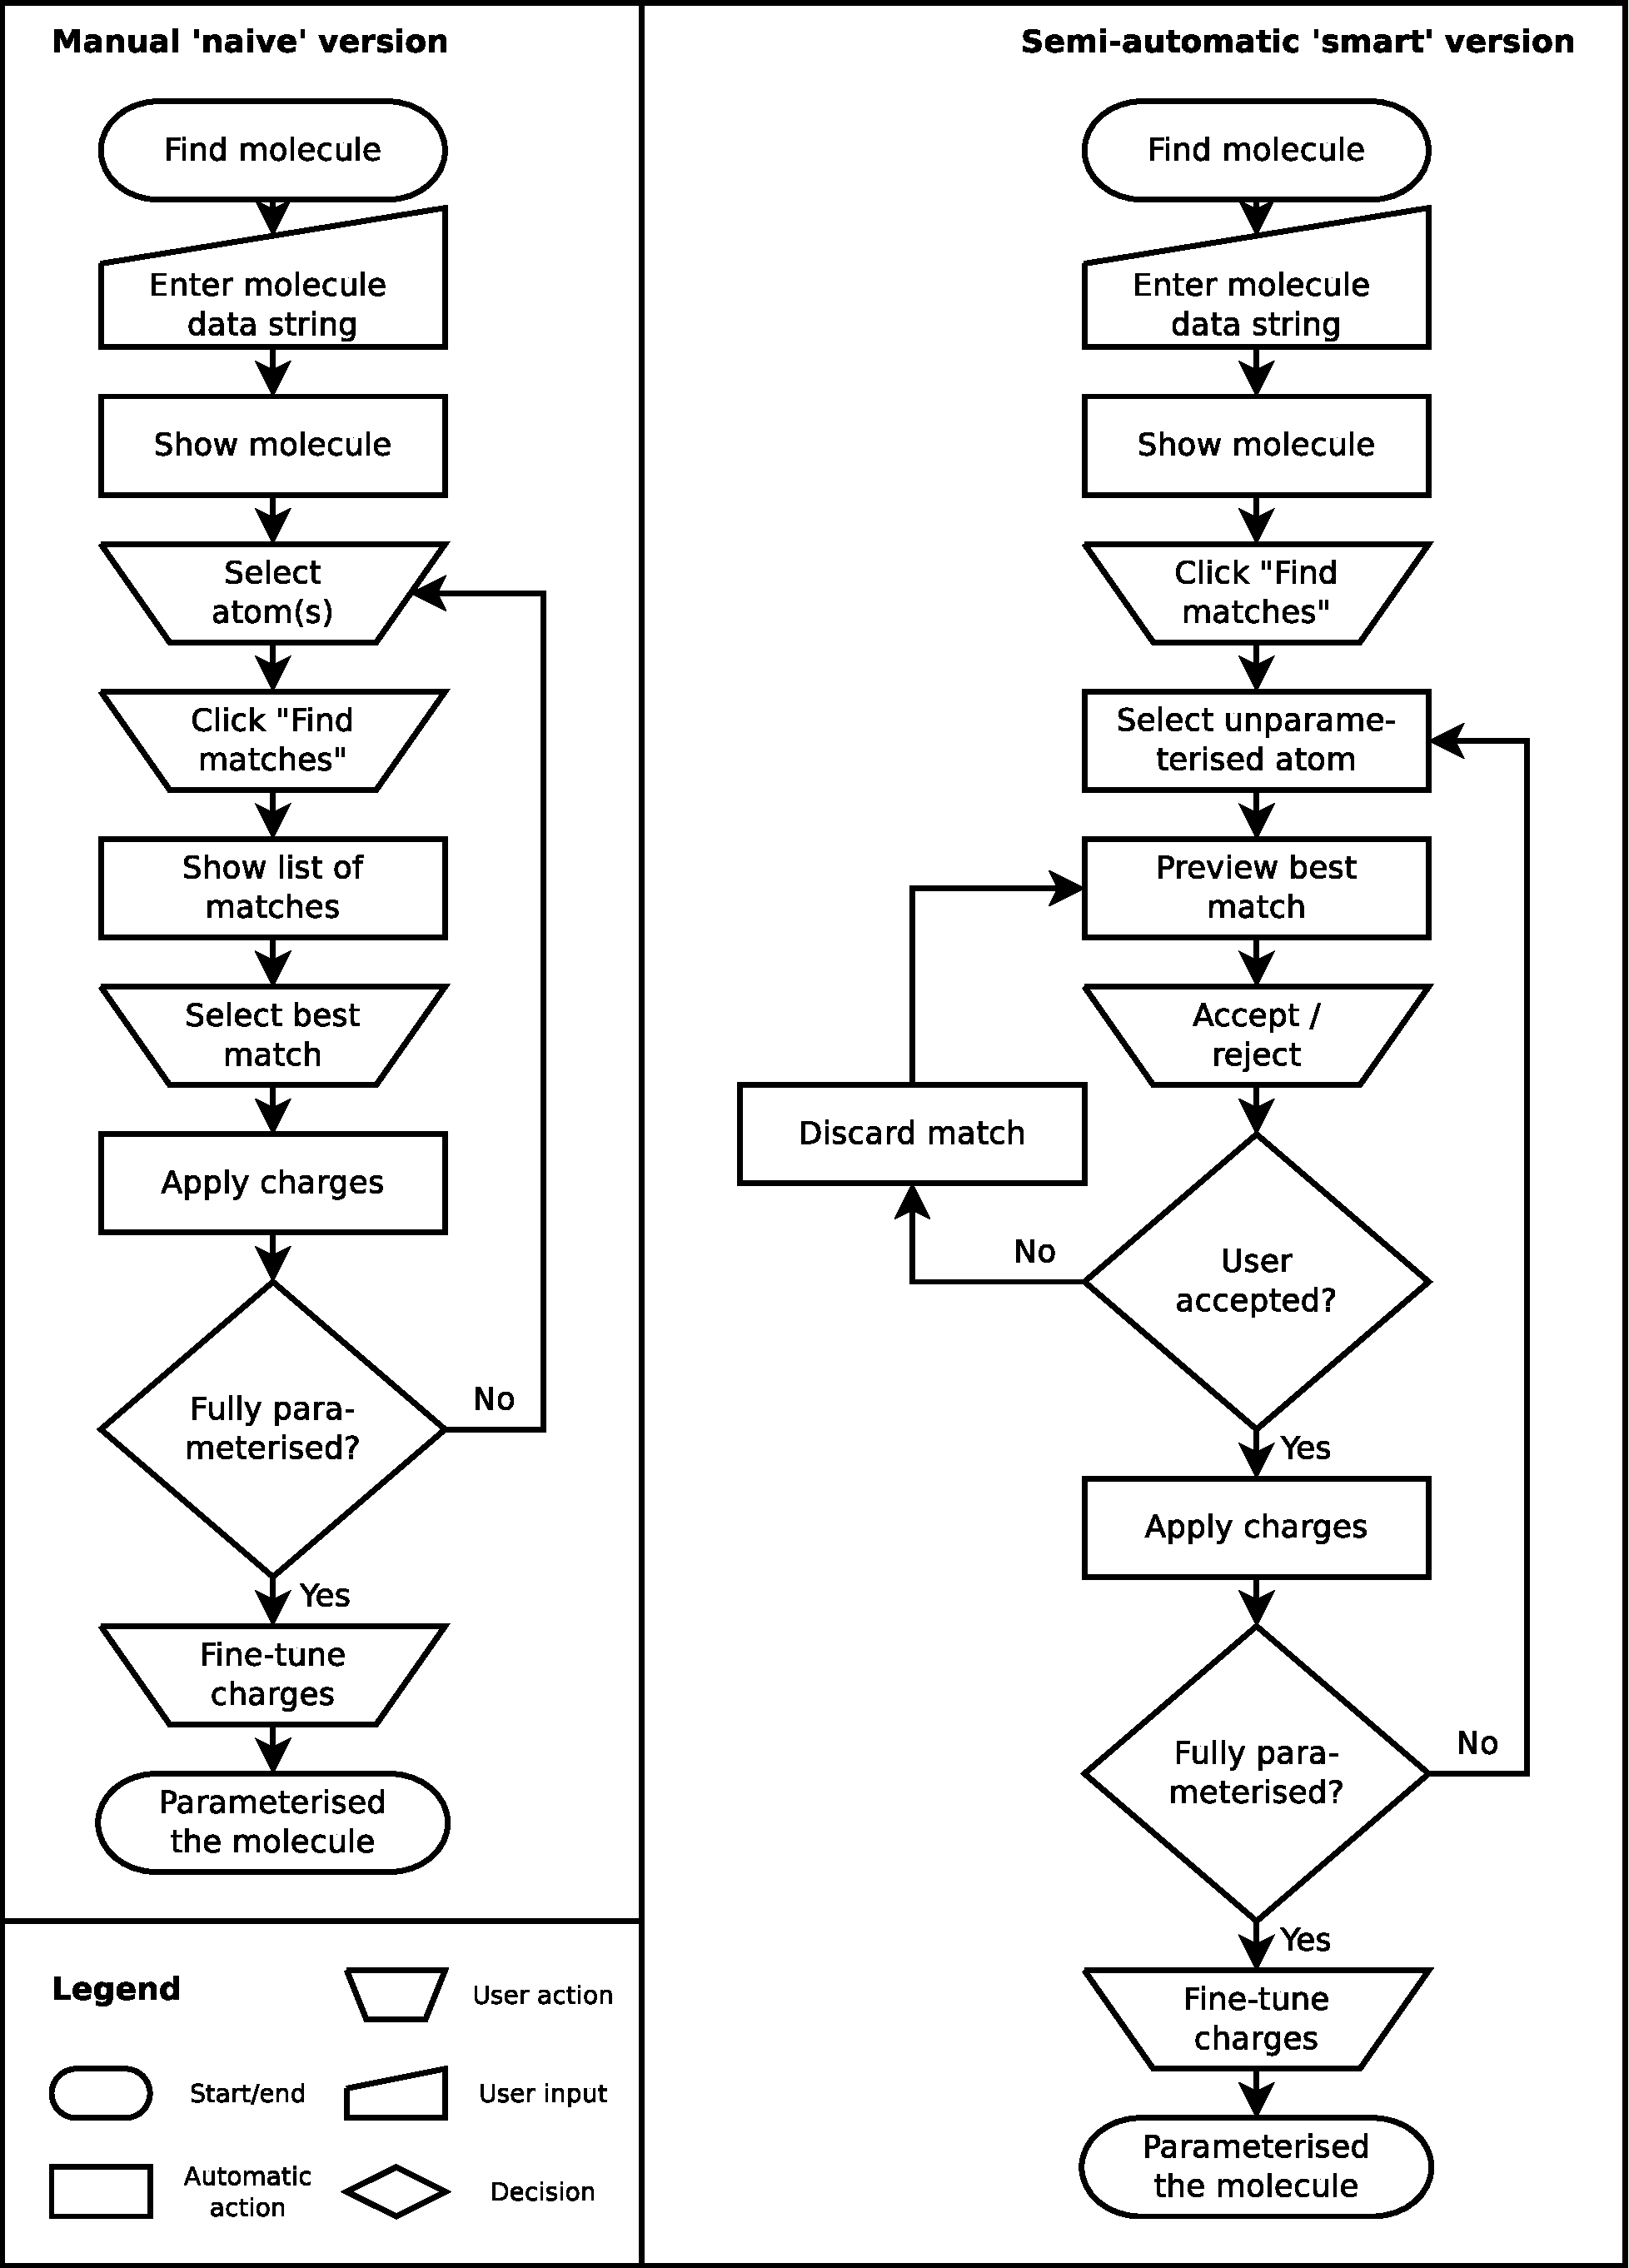
\includegraphics[width=.9\textwidth]{img/complete_id.pdf}
\caption{The two different interaction designs.}
\figlab{id_flows}
\end{center}
\end{figure}

%\begin{figure}[h!]
%\begin{subfigure}[t]{0.35\textwidth}
%\centering
%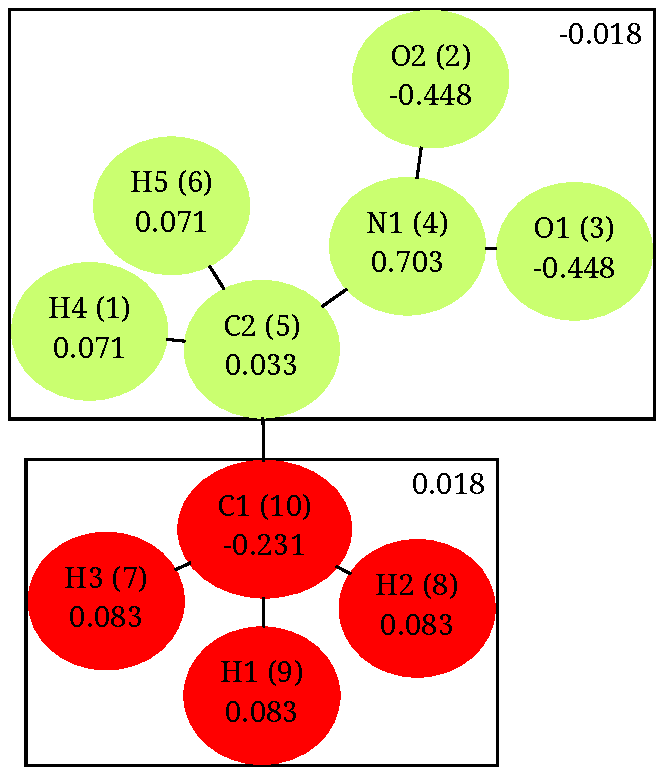
\includegraphics[width=100px]{img/partial_charges.pdf}
%\caption{The manual `naive' version.}
%\figlab{manual_id}
%\end{subfigure}\\
%\begin{subfigure}[t]{0.35\textwidth}
%\centering
%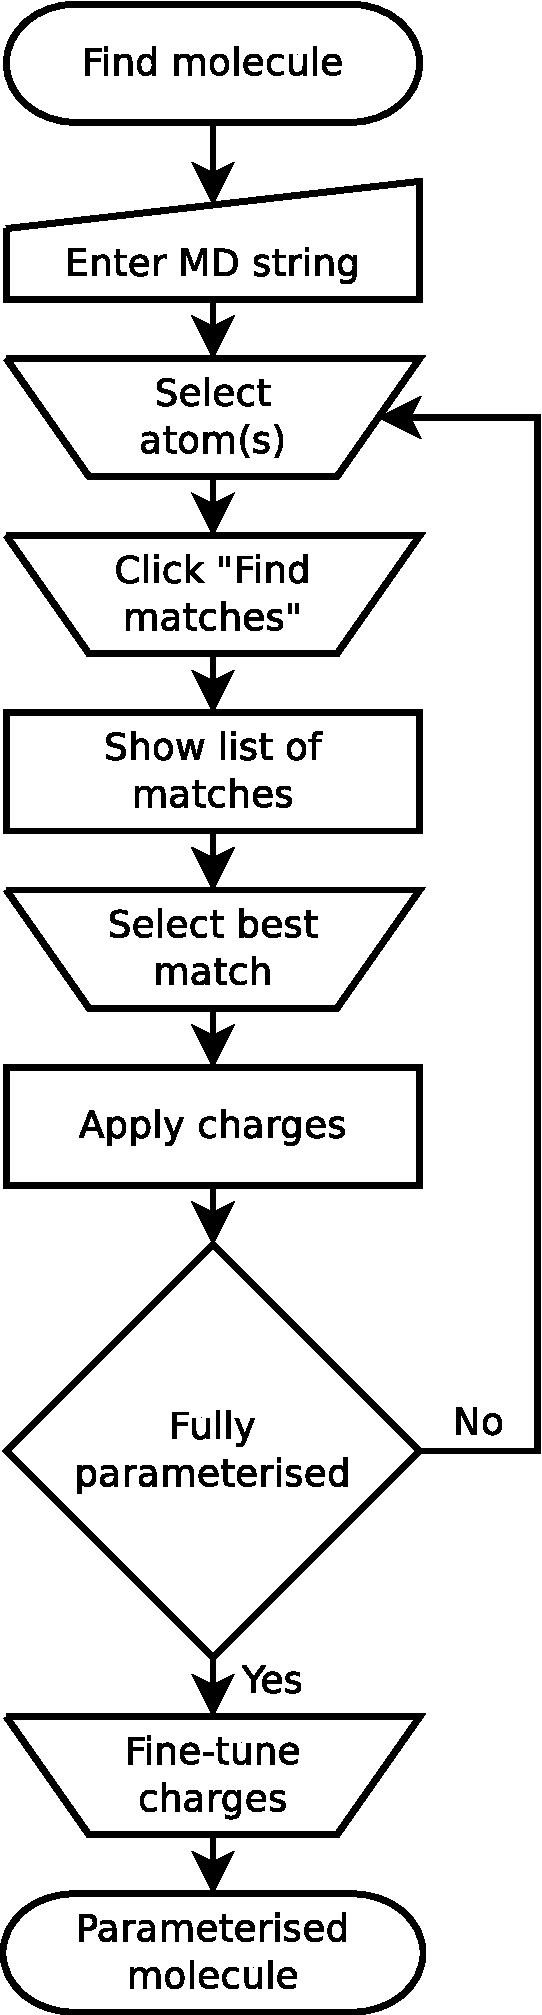
\includegraphics[width=123px]{img/manual_id.pdf}
%\caption{The manual `naive' version.}
%\figlab{manual_id}
%\end{subfigure}
%\begin{subfigure}[t]{0.65\textwidth}
%\centering
%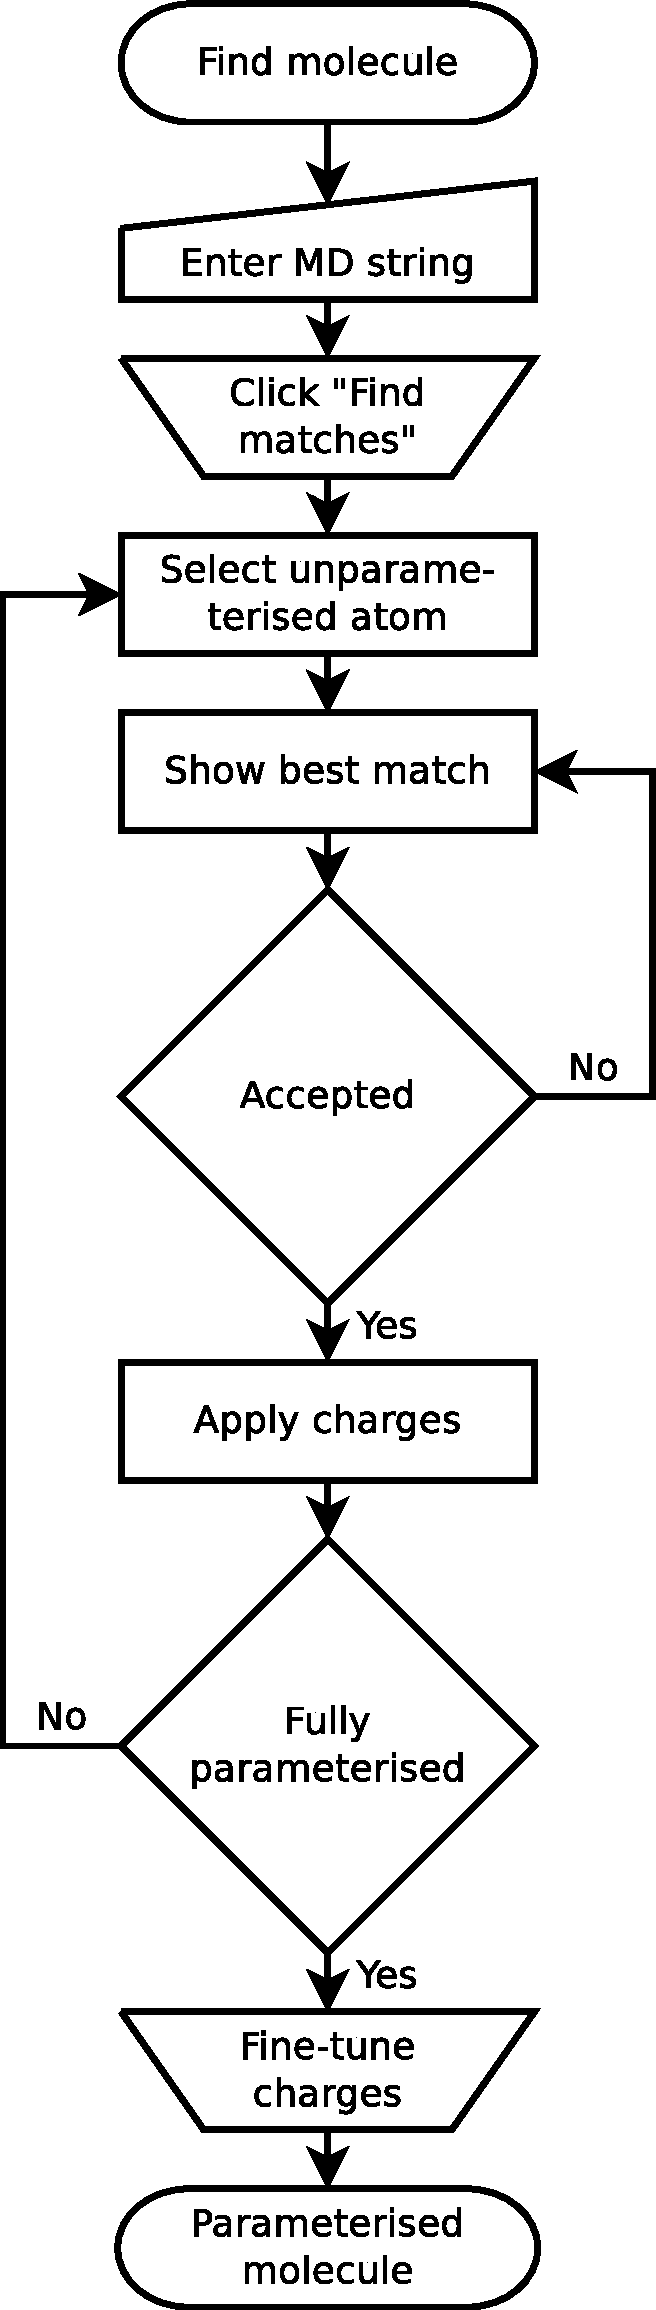
\includegraphics[width=220px]{img/semiauto_id.pdf}
%\caption{The semi-automatic `smart' version.}
%\figlab{semiauto_id}
%\end{subfigure}
%\caption{The two different interaction designs.}
%\figlab{id_flows}
%\end{figure}

Another possible variable in the tool is the way its users will interact with it and especially its degree of automation. Varying this degree has been the subject of several studies~(e.g.~\cite{payne2000varying, horvitz1999principles, marcus1987taking, norman1990problem}, see also \secref{id_automation}), all of which concluded the degree to which automation can be applied is highly dependent on the context of the system and sometimes even to the situation in which the system is used.

When implementing multiple versions of a tool with different levels of interaction, it is often decided to make three versions: a `naive' version without much automation, a `cooperative' version in which the user is given advise, and an `autonomous' version that only requires some parameterisation~(see~\cite{payne2000varying} and \secref{id_automation}). As it is considered hard to parameterise a molecule based on fragments of other molecules and little is known on what is the best way of doing this, an autonomous version of a tool that does this cannot yet be developed. The other two versions, however, seem to be perfectly implementable and both can be considered useful.

\Figref{id_flows} shows a naive and a cooperative interaction design for the tool that will be developed. Here, the cooperative design has been called the `smart' version to accentuate its differences with the naive version. The following sections will discuss these two interaction designs, the motivation behind them, their workings, and the hypotheses about them.

\subsection{Manual `naive' version}
In the naive version of the tool, the following steps should be followed to fully parameterise a molecule:
\begin{enumerate}[itemsep=.1em, parsep=.2em, topsep=0em]
\item The user enters a molecule data string (in \verb|SMILES|, \verb|InChI|, or other format);
\item The user selects a single atom or a set of \emph{connected} atoms;
\item The user clicks the ``Find matches'' button;
\item A list of matching fragments will be shown, ordered such that the highest rated match comes first and the lowest last. The user can browse through them, preview the result of selecting that match and, once he has found what he sees as the best match, select this match. Hereafter, the charges from that match will be assigned to the molecule;
\item
\begin{itemize}[leftmargin=0cm, itemsep=.1em, parsep=.1em]
\item[]{\bf Unparameterised atoms remain}:\\The user selects another atom / list of connected atoms. Back to step 3;
\item[] {\bf Molecule fully parameterised}:\\Continue to step 6;
\end{itemize}
\item When needed, the user can fine-tune the atom charges by selecting an atom and modifying its charge using an input field. In order to assist him in this process, the fragments that were matched to this atom \emph{and} have been selected will be shown;
\item The user is done.
\end{enumerate}

\noindent
In the matching process, it is possible that an already charged atom is present in another chosen fragment. In the case where these charges differ, the user will be asked to choose what should happen, which can be one of:
\begin{enumerate}[itemsep=.1em, parsep=.2em, topsep=0em]
\item Take the average of the two charges;
\item Keep the current value;
\item Take the new value;
\item Manually enter a value.
\end{enumerate}

\subsection{Semi-automatic `smart' version}
Using the semi-automatic version of the tool, the user should follow the following steps on order to fully parameterise a molecule:
\begin{enumerate}[itemsep=.1em, parsep=.2em, topsep=0em]
\item The user enters a molecule data string (in SMILES, InChI, or other format);
\item The user clicks the ``Find matches'' button. One of the atoms will now be automatically selected and matching fragments will be retrieved;
\item The highest rated match is previewed on the molecule. The user can either accept or reject this proposed match;
\item
\begin{itemize}[leftmargin=0cm, itemsep=.1em, parsep=.1em]
\item[]{\bf Rejected}:\\Remove this match from the list of matching fragments (the user \emph{can} go back to this one if he changes his mind). Back to step 3;
\item[] {\bf Accepted}:\\Assign the charges of the fragment to the molecule. Continue to step 5;
\end{itemize}
\item
\begin{itemize}[leftmargin=0cm, itemsep=.1em, parsep=.1em]
\item[]{\bf Unparameterised atoms remain}:\\Another unparameterised atom is automatically selected and similar fragments are retrieved. Back to step 3;
\item[] {\bf Molecule fully parameterised}:\\Continue to step 6;
\end{itemize}
\item The user can now fine-tune the charges by selecting an atom and modifying the charge using some input field, if he wants to do so. In order to assist him in this process, suggestions will be given on what atoms to fine-tune and to what value they should be adjusted;
\item The user is done.
\end{enumerate}

\noindent
In the matching process, it is possible that an already charged atom is present in another chosen fragment. In the case where these charges differ, the atom's charge will be automatically calculated from the two charges. Experimentation has yet to show the best way to do this, but, presumably, taking the average of the two will be a good solution.


\subsection{Pros and cons}
Both of the previously discussed methods have their benefits and disadvantages. Because of the limited level of user interaction in the `smart' version, parameterising a molecule can presumably be done much faster than in the `naive'  version. However, it is questionable how good the parameterisation will be, as the user is not really encouraged to explore a whole lot of fragments. Even though he will always be presented the highest rated match first, this match will not always be the best one. If, however, the user \emph{does} want to explore some other fragments, this might take more time than in the naive version, as only one fragment can be shown at a time.

The naive version may take up more time than the smart version, but it \emph{does} allow for a much higher level of control. The user can easily decide what atoms should be parameterised at which time and has a clear overview of the matching fragments. Furthermore, he can manually decide what should happen with overlapping fragments and can modify atom charges at any point in the process. If, however, the user lacks the experience of how to parameterise a molecule, or does not know what he is doing, he may not be able to make the right decisions, or even get lost in the large set of options. As the tool is aimed to be used by experienced scientists only, this should not be a problem, but experimentation will need to confirm that.


\section{Hypotheses}
\seclab{hypotheses}
Blah blah Brehmer and Munzer typololy, blahblah differences, blahblah \figref{id_typologies}\ldots

\begin{sidewaysfigure}[p]
\begin{center}
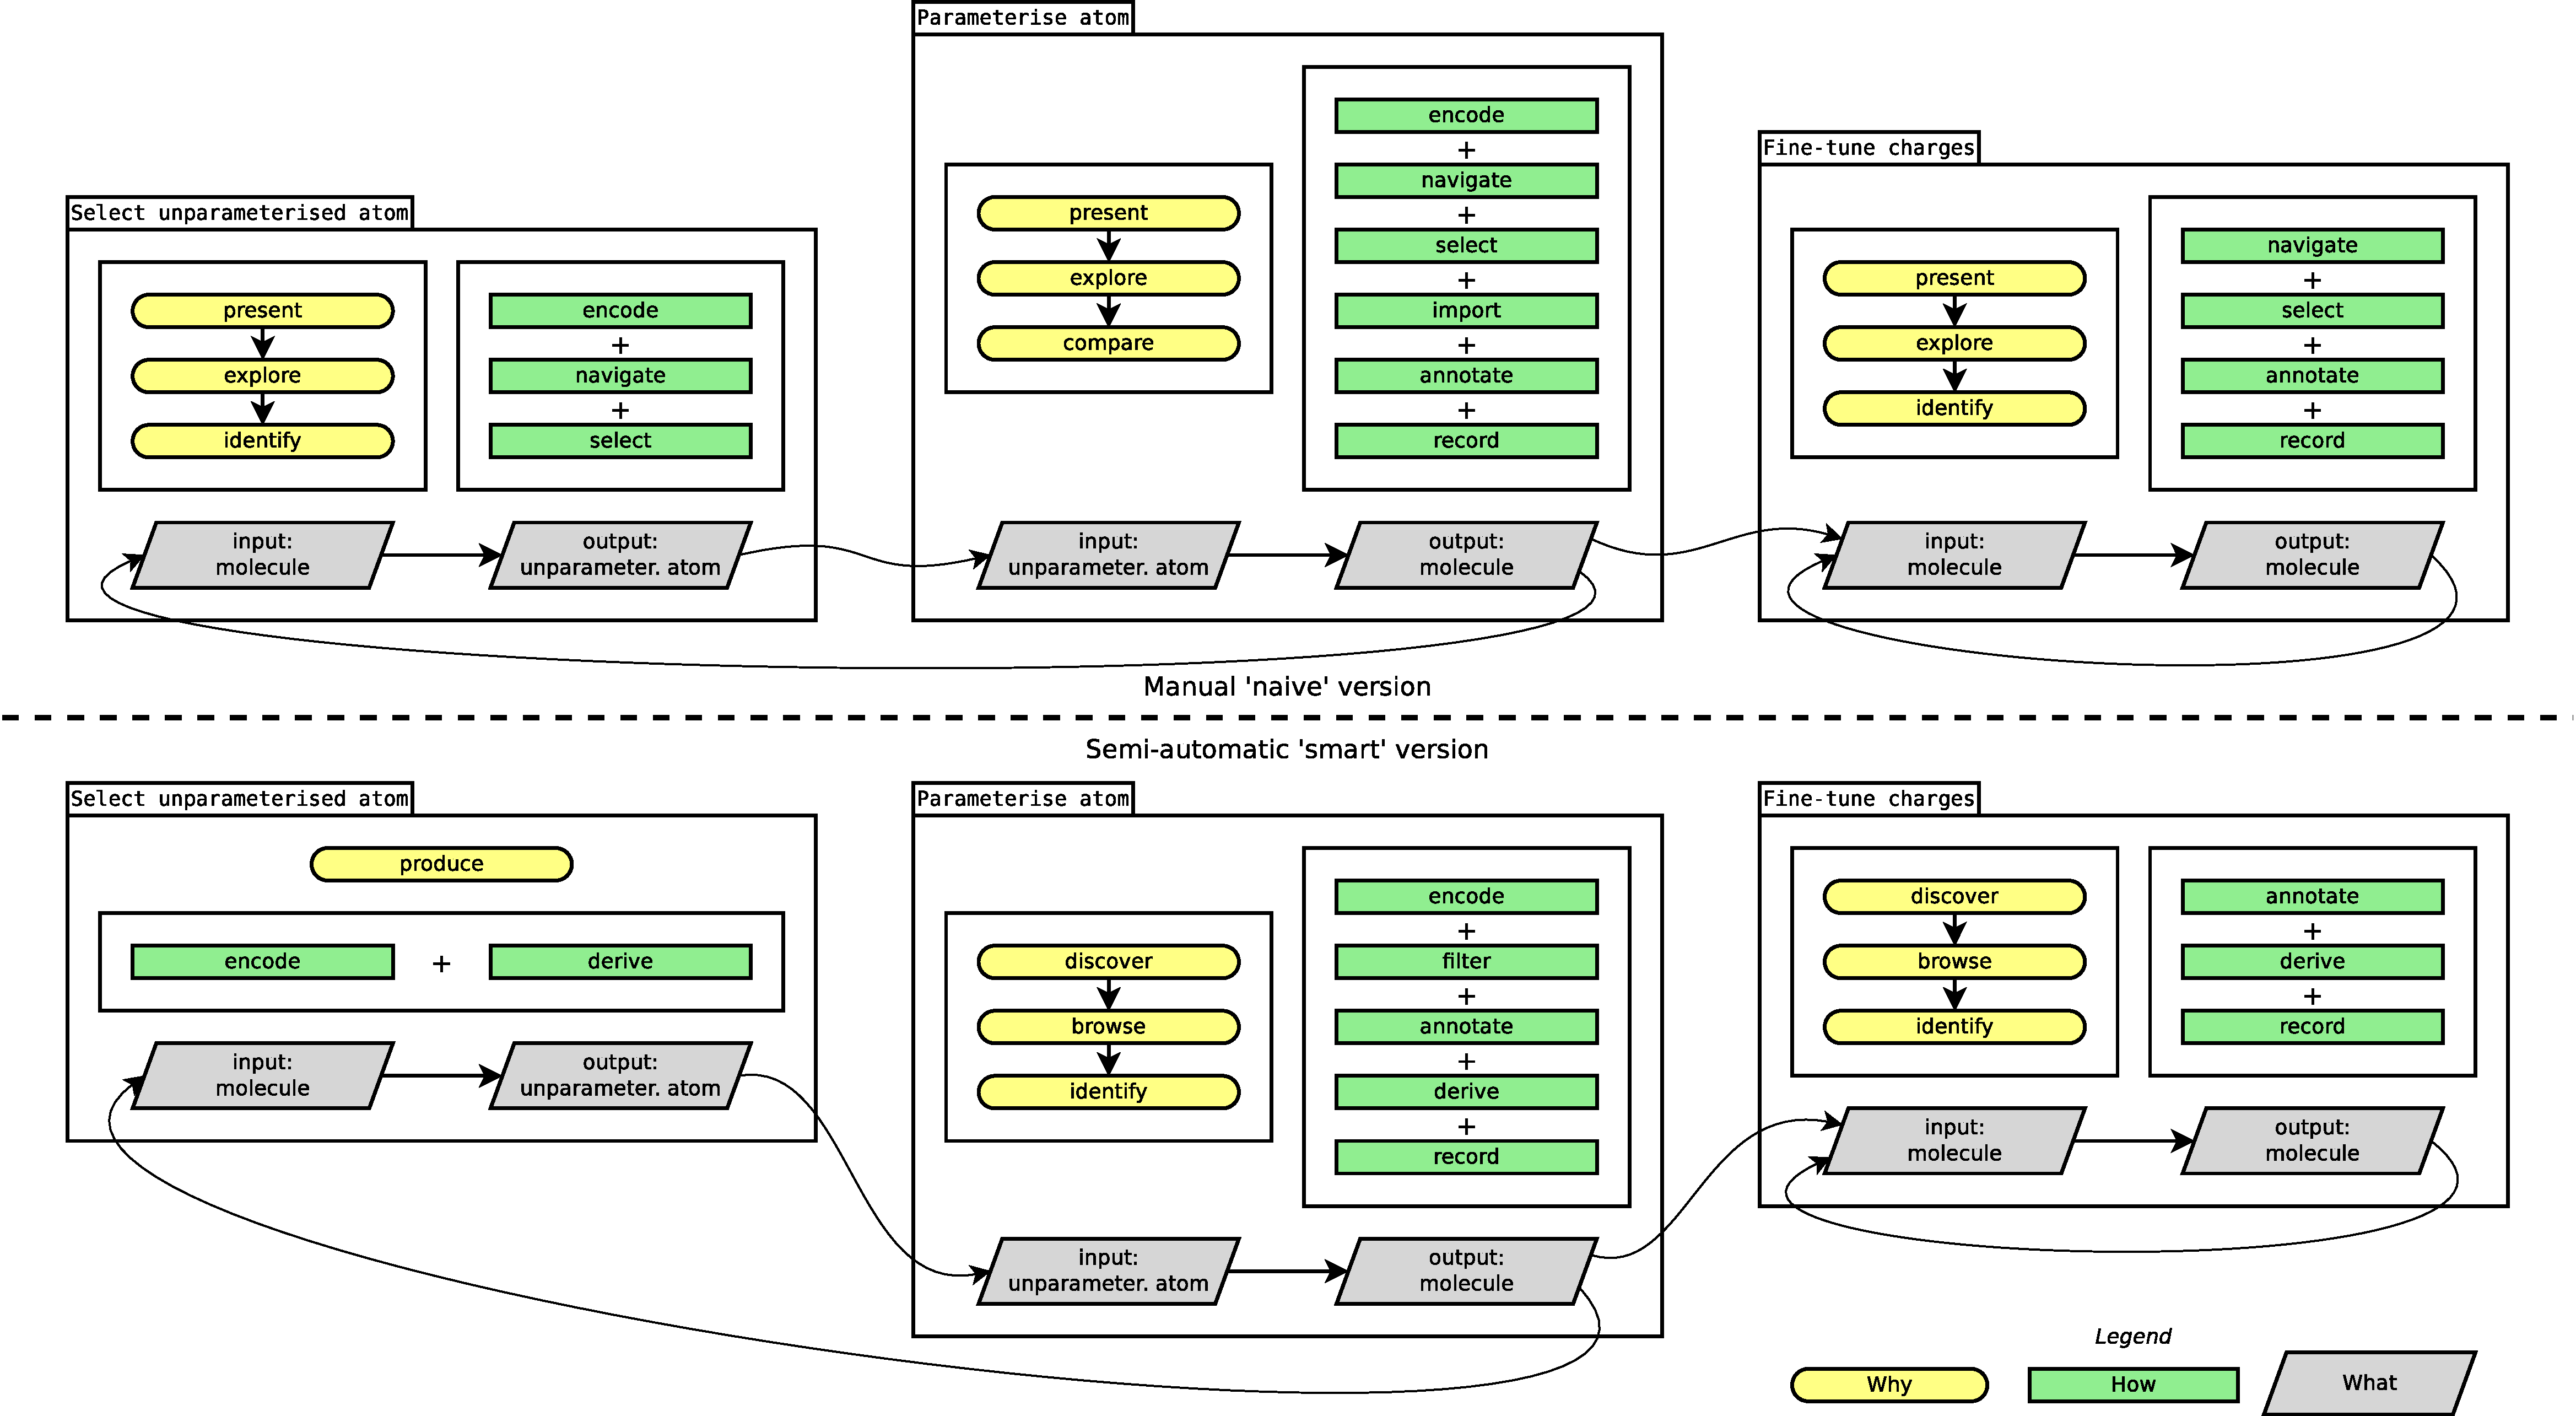
\includegraphics[width=\textwidth]{img/complete_typology.pdf}
\caption{Brehmer-Munzner Typologies of the two different interaction designs.}
\figlab{id_typologies}
\end{center}
\end{sidewaysfigure}

Blah blah these differences, blah blah one is better, blah blah because I say so\ldots


\section{Evaluation}
\seclab{evaluation}

To evaluate the project, both versions of the developed tool will be subjected to a number of user studies. Currently, however, the presumed user base is limited to only a small number of researchers. Luckily, project supervisors Klau and El-Kebir keep a close connection with most of those researchers, who work at VU University Amsterdam. They have shown some interest in the tool and are willing to participate in the user studies. Furthermore, as some of the researchers are also teaching, they can ask some of their students to evaluate the tool as well. This way, it is still possible to find enough test subjects, despite the fact that, initially, there are only a few targeted users.

In the user studies, the test subjects will be split up in two groups, where each subject is randomly assigned to a group and both groups are of equal size. One group will evaluate the naive version of the tool, the other will do the same for the smart version. Each group member will be asked to parameterise a few molecules of increasing size and complexity. The first one will be quite easy to complete, but the last one should be of such complexity that, theoretically, using the tool is beneficial over using conventional quantum mechanical calculations. It is in these last situations that the tool should show its true value.

During the tasks, the time required to complete the parameterisation will be measured. The difference between the time required in the two implementations will help deciding which of the two implementations is better, but, for both tools, completing the parameterisation should definitely not take hours to finish. Furthermore, users should never be annoyed or willing to stop parameterising.

Besides time, the user will also be scored on his performance. In order to do this, the molecules that the user will be asked to parameterise should already have been parameterised using the conventional quantum mechanical calculations. This way, the user's results can be compared to the outcomes of the calculations to establish his score. The smaller the difference between the two, the better the performance of the user will be graded. Of course, there will always be a small difference between the manual and calculated ways, as the manual assignment cannot be as precise as the calculated one is. However, as long as the difference is small, the developed tool can be considered useful to speed up atomic charge assignment.

After completing their tasks, the users will be asked to answer a number of questions about the tool. These will mainly be about how they like the design and if they can see themselves using it, but will also ask them for suggestions on things that can be improved or added. This way, their experiences can be used to further improve the tool, and to make it a tool they really like using.


\section{Time line}
\seclab{timeline}

There is a period of five months available for this project, which will be spent as follows:

\noindent
\begin{tabular}{r|l}
\textbf{Sep-Nov} & Project plan and literature study\\
\textbf{Oct-Jan} & Iteratively design, implement and validate the tool\\
\textbf{Jan-Feb} & Thesis\\
\textbf{Feb} & Thesis defence
\end{tabular}

\noindent
Note that in September and October, the project will only be worked on three days per week. From November to January, the project will be worked on full time.

User studies with real potential application users will hopefully be held in the second half of December, but might, due to the holidays, be delayed to the first half of January. Having the user studies before the end of the implementation phase allows for an additional period in which any flaws discovered by the user studies can be fixed. However, this also means there should be a working version of the tool before the end of December. During the implementation phase, frequent progress meetings with the project supervisors will be organised, to make sure flaws are discovered at an early stage and can be quickly solved. This takes away the need for a testing, fixing and improving phase at the end of the project.
